\chapter{Experiments and results}
\label{ch:Experiments}

This chapter presents the results attained by applying the EDM process to the educational data set of the IMD's students and the proposed web application that will use the models selected after the analysis. Before showing the results it is important to understand how the academic performance is done in the IMD's IT technical course: the students' final grade is a combination of four distinct tasks. Two of these tasks are done at the end of the course and combined weighs 65\% of the final grade. The other two tasks are done and graded weekly, combining 35\% of the final grade. The analysis done in this research uses only those weekly grades.

To give an overview of the data set, descriptive statistics are shown in table \ref{tab:da}, and a histogram of the students' final score, grouped by Pass (True) or Fail (False), is shown in figure \ref{fig:mm}. It can be noticed that it already exists a balance in the data set between classes Pass and Fail. This is important because the classifiers could become biased towards the majority class if the data set is imbalanced. Grades have a peak of occurrences around 5, which is the minimum grade for passing, and another peak around 0, most likely indicating those students who gave up the course.

\begin{table}[ht]
\centering
\begin{tabular}{ccc} \hline
\textbf{Final result} & \textbf{Number of students} & \textbf{Percentage of students} \\ \hline
Pass                  & 3427                        & 56.47\%                         \\
Fail                  & 2642                        & 43.53\%                         \\ \hline
\end{tabular}   
\caption{Final situation of students in classes}
\label{tab:da}
\end{table}

\begin{figure}[hbt!]
	\centering
  	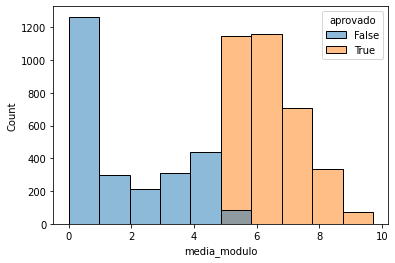
\includegraphics[scale=.43]{Resultados/mm.png}
  	\caption{Students' final score}
  	\label{fig:mm}
\end{figure}

The problem of predicting students' end-of-term results is an example of a classification problem. In this work, the results for a binary problem (final result can be either 'Pass' or 'Fail') and also for a 3-class problem (final result can be either 'High risk', 'Middle risk', or 'No risk') were calculated.

For the 3-class problem, the final students' grades were grouped in 3 classes determined by applying the $k$-means algorithm. The centroids of the three classes are 0.78, 4.92, and 7.06. Details about the classes' balance using those groups are shown in table \ref{tab:3c}.

\begin{table}[htb]
\centering
\begin{tabular}{ccc} \hline
\textbf{Class} & \textbf{Number of students} & \textbf{Percentage of students} \\ \hline
High risk                & 2202                        & 36.43\%               \\
Middle risk              & 1760                        & 29.12\%               \\
No risk                  & 2082                        & 34.45\%               \\ \hline
\end{tabular}
\caption{3-class frequency distribution}
\label{tab:3c}
\end{table}

\section{Data preprocessing}
The first action in the preprocessing stage was to select the most relevant features. The original data set had a total of 127 features, but some of these features are either a combination of other attributes or are scores determined only at the end of the course. As the focus of this research is only on the weekly grades and attendance data, it was decided to reduce the data set.

In addition, features of weeks 19 and 20 (the last two weeks in the data set) were dropped due to the amount of missing data, as seen in table \ref{tab:featmiss} with features' description in table \ref{tab:Dataset2}. 

\begin{table}[hbt]
\centering
\resizebox{8cm}{!}{%
\begin{tabular}{cc} \hline
\textbf{Feature} & \textbf{Percentage of missing values} \\ \hline
pp17 & 2.58\% \\
pv17 & 2.37\% \\
f17 & 2.58\% \\
pp18 & 8.76\% \\
pv18 & 8.55\% \\
f18 & 8.76\% \\ \hline
pp19 & 39.36\% \\
pv19 & 39.14\% \\
f19 & 39.36\% \\
pp20 & 77.73\% \\
pv20 & 77.73\% \\
f20 & 77.73\% \\ \hline
\end{tabular}%
}
\caption{Percentage of missing values of last weeks' features}
\label{tab:featmiss}
\end{table}

Following, two features were replaced to represent the classes of the problem, either for the binary or 3-class problem. In the former case, the final result class was changed from a nominal variable (with distinct classes to indicate if the student passed or failed) to a binary (only classes 'Pass' and 'Fail'). In the latter case, the final grade was changed from a continuous variable to a nominal variable with three distinct classes ('High risk', 'Middle risk', or 'No risk').

To sum up, after the preprocessing, the reduced data set, used by the classifiers, had a total of 56 features that can be seen in detail in table \ref{tab:Dataset2}.

\begin{table}[hbt]
\centering
\resizebox{\textwidth}{!}{%
\begin{tabular}{lll}
\hline
\bf{Feature} &
  \bf{Type} &
  \bf{Description} \\ \hline
\begin{tabular}[c]{@{}l@{}}pp1 pp2 pp3 pp4 pp5\\ pp6 pp7 pp8 pp9 pp10\\ pp11 pp12 pp13 pp14 pp15\\ pp16 pp17 pp18 \end{tabular} &
  Numerical {[}0.0, 10.0{]} &
  \begin{tabular}[c]{@{}l@{}}Score in activities made in the classroom.\\ Each number indicates the week of the activity.\end{tabular} \\ \hline
\begin{tabular}[c]{@{}l@{}}pv1 pv2 pv3 pv4 pv5\\ pv6 pv7 pv8 pv9 pv10\\ pv11 pv12 pv13 pv14 pv15\\ pv16 pv17 pv18 \end{tabular} &
  Numerical {[}0.0, 10.0{]} &
  \begin{tabular}[c]{@{}l@{}}Score of students' participation in the virtual learning environment.\\ Each number indicates the week of the activity.\end{tabular} \\ \hline
\begin{tabular}[c]{@{}l@{}}f1 f2 f3 f4 f5\\ f6 f7 f8 f9 f10\\ f11 f12 f13 f14 f15\\ f16 f17 f18 \end{tabular} &
  Numerical {[}0.0, 1.0{]} &
  \begin{tabular}[c]{@{}l@{}}Attendance of the student in a week.\\ Each number indicates the week.\end{tabular} \\ \hline
nivel\_de\_risco &
  Nominal & \begin{tabular}[c]{@{}l@{}}It can be one of three classes (no risk, middle risk or high risk).\\ Based on the students' final grade.\end{tabular} \\ \hline
aprovado &
  Nominal &
  \begin{tabular}[c]{@{}l@{}}Final result of the student in the full course.\\ 'True' if the student passed the course, 'False' otherwise.\end{tabular} \\ \hline
\end{tabular}%
}
\caption{Students' academic performance reduced data set}
\label{tab:Dataset2}
\end{table}

The next action was dealing with missing data. In this step data from students that canceled the course was removed. Most of the students' dropping out happened in the 2020.1 semester, an atypical semester that, due to the COVID-19 pandemic, was not done in the usual hybrid format. The semester started as usual but by the 4th-week classes were stopped, returning 12 weeks later with only online classes. The students were given the choice to continue in this new format or to drop out of the course. This action implied losing 247 of the 6316 samples (3.91\% of the data set). Data is shown in detail in table \ref{tab:dropouts}.

\begin{table}[hbt]
\centering
\begin{tabular}{cccc}
\hline
\textbf{Semester} & \begin{tabular}[c]{@{}c@{}}\textbf{Number of}\\ \textbf{students}\end{tabular} & \begin{tabular}[c]{@{}c@{}}\textbf{Number of}\\ \textbf{dropped out}\\ \textbf{students}\end{tabular} & \textbf{Dropout rate} \\ \hline
2015.1 & 1351 & 0 & 0.00\% \\ 
2016.1 & 1160 & 0 & 0.00\% \\ 
2017.1 & 1076 & 0 & 0.00\% \\ 
2017.2 & 697 & 0 & 0.00\% \\ 
2018.1 & 639 & 0 & 0.00\% \\ 
2019.1 & 634 & 7 & 1.10\% \\ 
2020.1 & 759 & 240 & 31.62\% \\ \hline
\end{tabular}
\caption{Students' dropout rate}
\label{tab:dropouts}
\end{table}

The remaining missing values were updated with the mean value for the feature, as this is a usual way of dealing with missing data. Finally, the last action was to scale the data so that all features share the same range. This was done because some of the algorithms used need it to work properly. So, all numeric features were scaled to the [0, 1] interval.

\section{Data analysis}

In related works \cite{sokkhey2020developing} \cite{akccapinar2019using} \cite{soule2017predicting}, numerous algorithms are cited as able to solve the problem of predicting the students' final result. So, in this work, the following algorithms were selected: Naive Bayes, KNN, Random Forest, and Logistic Regression. The performance of these selected algorithms was initially compared based on accuracy, as it is the usual approach in classification problems with a balanced data set.

The performance results were obtained using a 4-fold cross-validation method in all analyses. Finally, before obtaining the scores of the classifiers' performance, a grid search was done to optimize the parameters of the algorithms. The final parameters, used in all analyses, are shown in table \ref{tab:param}. To clarify, the $p=1$ parameter in the KNN classifier indicates that the distance measure is the Manhattan distance.

\begin{table}[ht]
\centering
\begin{tabular}{cc}
\hline
\textbf{Classifier}                                & \textbf{Parameters}                                                                                  \\ \hline
KNN & \begin{tabular}[c]{@{}l@{}}weights='distance'\\ p=1\\ n\_neighbors=10\end{tabular}                   \\ \hline
Logistic regression                                & \begin{tabular}[c]{@{}l@{}}max\_iter=500\\ solver='newton-cg'\end{tabular}                           \\ \hline
Naive Bayes                                        &                                                                                                      \\ \hline
Random forest                                      & \begin{tabular}[c]{@{}l@{}}max\_features=None\\ criterion='entropy'\\ n\_estimators=200\end{tabular} \\ \hline
\end{tabular}
\caption{Classifiers' parameters}
\label{tab:param}
\end{table}

\subsection{Results}
The first results summarize the classifiers' accuracy using all data up to a given week, in other words, all available data of grades and attendance for any given week is used to train and test the model. These results are exhibited in figures \ref{fig:ab} and \ref{fig:a3c}, and it shows that the results were similar with a slight advantage to the Logistic Regression model that obtained better results in the early weeks. For this reason, this classifier was chosen to further analysis.

The results of the Logistic Regression classifier are shown in more detail in table \ref{tab:lr}, with multiple performance metrics. The 3-class results are the mean of each metric for each label. These results show that in both binary and 3-class problems the F-Measure is even better than accuracy and that in the binary problem the recall always yields the best results between the different metrics. The high recall measures could indicate that the models are good at minimizing false negatives.

The second results were obtained by using the Logistic Regression classifier again but with different subsets of attributes from the reduced data set. This was done to see the difference in results in comparison to using the full set of features. The subsets of attributes with its description are detailed in table \ref{tab:fd} and the results are shown in figures \ref{fig:lrb} and \ref{fig:lr3c}. These results indicate that the model using all grades' features and leaving the attendance out is close in performance to the model using the full set of features. For this reason, the final chosen model was the Logistic Regression classifier using only the grades' features.

\begin{table}[htb]
\centering
\begin{tabular}{cc} \hline
\textbf{Set of features} & \textbf{Description} \\ \hline
pp+pv+f & Full set of features. \\ \hline
pp+pv & Combines all grades' features. \\ \hline
pp & Features of grades' score in activities made in the classroom. \\ \hline
pv & \begin{tabular}[c]{@{}c@{}}Features of grades' score in activities \\ made in the virtual learning environment.\end{tabular} \\ \hline
f & Features about attendance. \\ \hline
\end{tabular}
\caption{Description of the features' set}
\label{tab:fd}
\end{table}

Related to the 3-class Logistic Regression models, a confusion matrix was built (see figure \ref{fig:3ccm}). This confusion matrix is the sum of all confusion matrices of the models, using only grades' features, of the 18 weeks of the course schedule. It presents the real observed values in the $y$-axis and the predicted values by the model in the $x$-axis. It can be seen that the two biggest errors are, respectively, a 'Middle risk' student being classified as 'No risk', and a 'No risk' student being classified as 'Middle risk'. Thus, the confusion in the models' classification is greater in the zone between the classes 'No risk' and 'Middle risk'.

\begin{figure}[htb]
	\centering
  	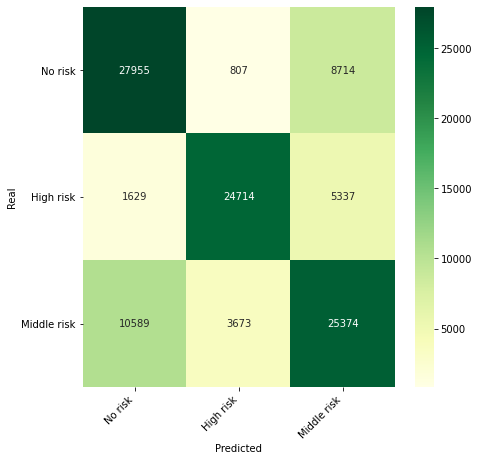
\includegraphics[scale=.7]{Resultados/3classes_confusion_matrix.png}
  	\caption{Confusion matrix of the Logistic Regression 3-class models}
  	\label{fig:3ccm}
\end{figure}

After these results, because of the better performance, the binary Logistic Regression classifier was chosen to be integrated into the web application. The models were built dropping the scaling in features to the [0, 1] interval, this way, all attributes stayed in the [0, 10] interval. The full set of models is shown in appendix \ref{ch:Models}. The default class ($y=1$) indicates that the student is classified as approved in the course.

Given these models, some interpretations could be made, such as the current week's coefficients are usually the greatest and that between type 1 grade (pp), activities made in the classroom, and type 2 grade (pv), activities in the virtual learning environment, the latter usually weigh more. Thus, the type 2 grade could have more influence on the students' chances of passing. Also, it is possible to plot the Logistic Regression function fixing all but one feature, this way it can be seen what impact one specific grade has in the students' chances, according to the model.

For example, using the week 4 model and the median values of the attributes of previous weeks the figure \ref{fig:w4m} plot can be made. This graph indicates that if the student receives a 3.5 or more in type 1 grade (pp) chances are in his or her favor, same for type 2 grade (pv) starting at 6.55.

\begin{figure}[htb]
	\centering
  	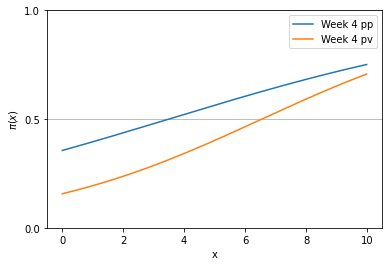
\includegraphics[scale=.7]{Resultados/week4models.png}
  	\caption{Logistic Regression function of week 4 model}
  	\label{fig:w4m}
\end{figure}

\section{Web system design}
The proposed web application's purpose is to act as an early warning system to help students and teachers. This tool can benefit the former by having a way to visualize if his/her current weekly grades are good enough to succeed in the course, while the latter benefits by easily spotting the underperforming students, enabling possible interventions.

Figure \ref{fig:sigaa_aluno} shows the current web page that the students have to see the weekly grades. It is just a table crossing week and type of grade. Using only the information shown on this page, there is no obvious way to know if the student is performing well in the course, in any given week. Thus, the suggested web system aims to be an improved version of that page, showing not only the grades but feedback of the student performance.

\begin{figure}[htb]
	\centering
  	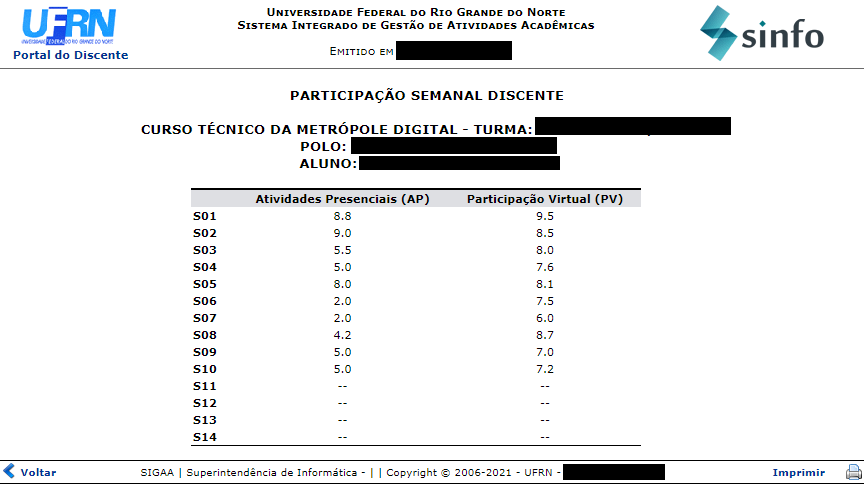
\includegraphics[scale=.7]{Resultados/sigaa_aluno.png}
  	\caption{SIGAA student page of weekly grades}
  	\label{fig:sigaa_aluno}
\end{figure}

\subsection{Architecture}

Three main components were necessary to the development of the application: (1) a source of the educational data, (2) the models that predict academic performance, and (3) a server to integrate the two previous components and exhibit the results to the users.

Firstly, the source of the data should be the official University's API\footnote[1]{\hspace{1mm}University's API services available in: \url{https://api.ufrn.br/servicos.html}} but as the required data of students' grades were not available at the time of this research, a mock API server was built to replace the official API in the main server. The mocked server simulates only three services: get data from the logged-in user, the users' classes, and the users' grades in a class.

Secondly, the Logistic Regression binary models, from week 1 to 18, were exported and added to the main server. These models are small files that were fast to build and are fast to make predictions. This was expected as the Logistic Regression models are easy to represent as they are essentially storing the intercept and coefficients of the models.

Finally, the main server was built. This server uses the two previous components to power the web system's dashboards.

In summary, the server is structured as shown in figure \ref{fig:server}.

\begin{figure}[htb]
	\centering
  	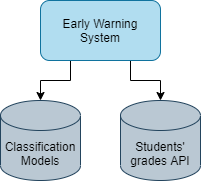
\includegraphics[scale=.7]{Imagens/server-model.png}
  	\textsf{\caption{Web server architecture}
  	\label{fig:server}}
\end{figure}

\subsection{Dashboards}

The first system page, the login, should use the unified authentication of the University's API applications (see figure \ref{fig:login}). After the user is logged on, there are two possible use cases:

\begin{enumerate}
    \item Student dashboard
    
The server verifies the class that the student is enrolled then queries the API to obtain all the student's weekly grades. Next, the models classify the student in each week as either likely or not to pass the course. This information is shown in the student dashboard, with cards from all weeks of the course that were graded. Those cards show the scores and performance indicators in each week (see figure \ref{fig:webs}). The indicators can be green, indicating that the student is likely to succeed, otherwise, it is red.

    \item Teacher dashboard

The server verifies the class that the teacher is responsible then queries the API to obtain all the teacher's weekly class grades. Next, the models classify each student in each week as either likely or not to pass the course. This information is shown in the teacher dashboard, with a single table crossing data from students and weeks of the course (see figure \ref{fig:webp}). This table also shows indicators that work the same way as it is for the student.
\end{enumerate}

\begin{figure}[!htb]
   \begin{minipage}{0.48\textwidth}
     \centering
     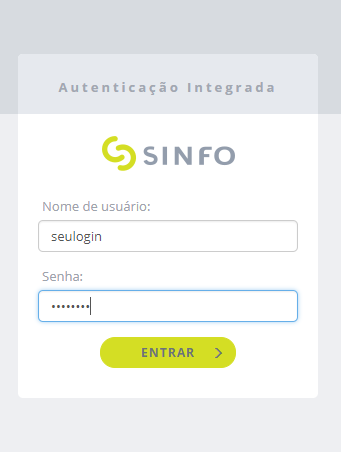
\includegraphics[width=.9\linewidth]{Imagens/login.png}
     \caption{Login page}\label{fig:login}
   \end{minipage}\hfill
   \begin{minipage}{0.48\textwidth}
     \centering
     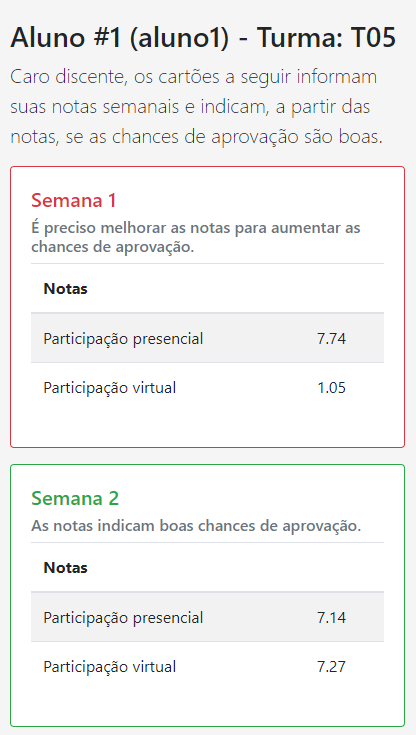
\includegraphics[width=.8\linewidth]{Resultados/web-student.png}
     \caption{Student dashboard}\label{fig:webs}
   \end{minipage}
\end{figure}

\begin{figure}[htb]
	\centering
  	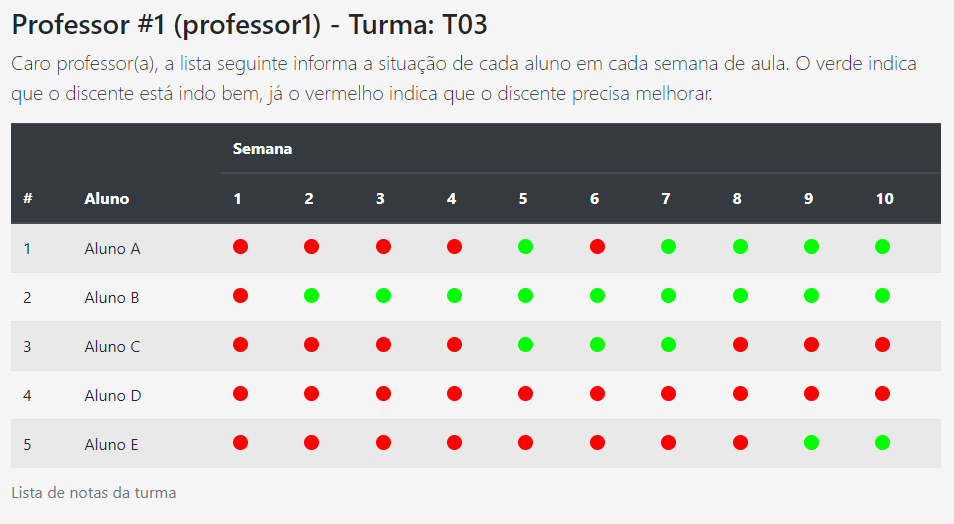
\includegraphics[scale=.6]{Resultados/web-teacher.png}
  	\textsf{\caption{Teacher dashboard}
  	\label{fig:webp}}
\end{figure}

